\section{Graphs}
A \textit{graph} is an 
ordered pair $G = (V,E)$ comprising of a set of vertices, $V$, and a set of edges or 
lines, $E$.  Every edge $e \in E$, is an unordered pair of distinct vertices $u,v \in V$ (the edge represents their adjacency, $e = \{ u,v\}$). With this definition of a graph, there 
are 
no loops (self adjacent vertices, $\{v,v\}$) or multi-edges (several edges between the same pair of 
vertices).

A motivation for using graphs is modeling physical objects like molecules.  This requires an 
embedding into the plane or $\bbr^3$.  An \textit{embedding} of the 
graph $G = (V,E)$ is an injective mapping $\Pi : V \mapsto \bbR^{2}$ (see Figure 
\ref{fig:graph1-1}). 

\begin{figure}[!htbp]
\begin{center}
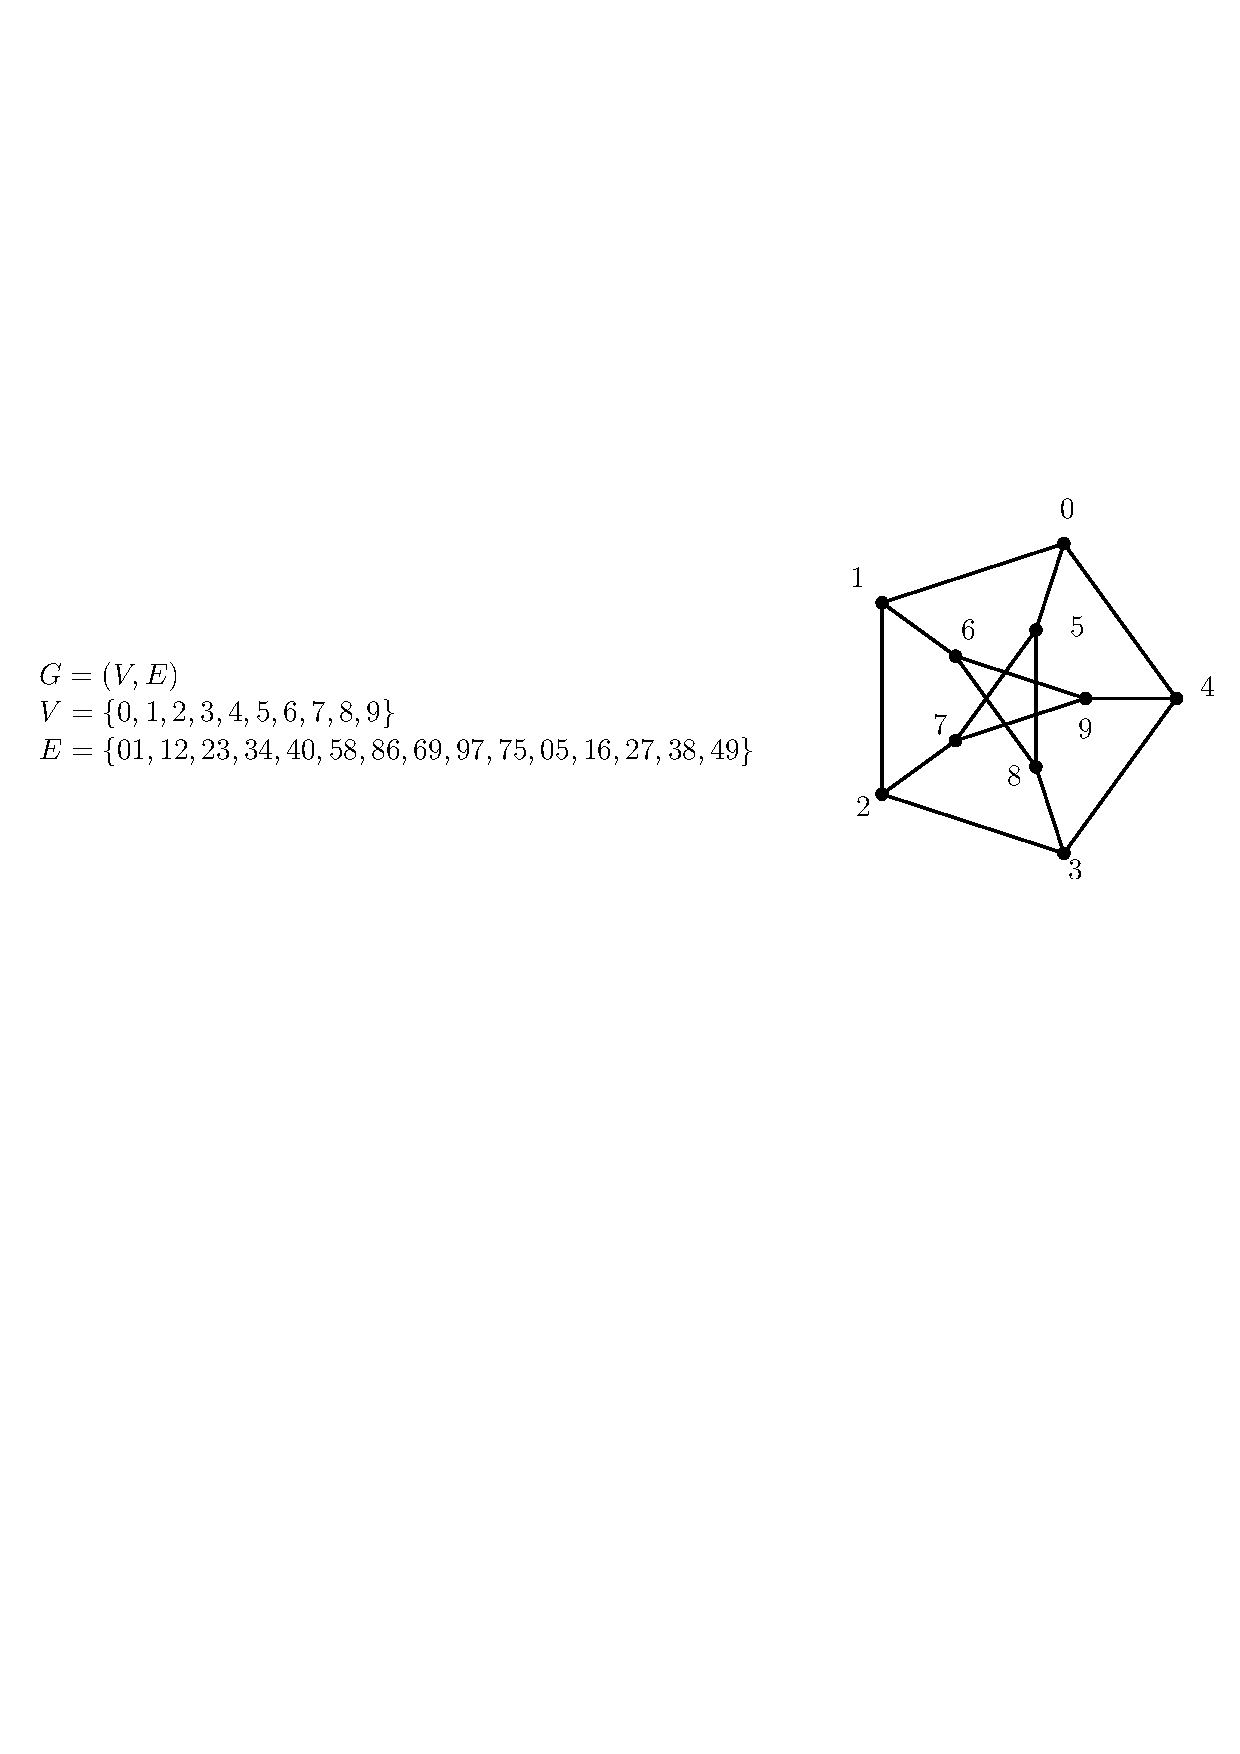
\includegraphics[scale=.5]{graphics/PetersonGraphExample.pdf}
\caption{An embedding of the Peterson graph.}\label{fig:graph1-1}
\end{center} 
\end{figure} 
\subsubsection{Edge Crossings}
We define \textit{plane embeddings} of a graph to be an embedding where the following degenerate 
configurations 
do not occur:
\begin{itemize}
\item[\rn{1}] the interiors of two or more edges intersect, or
\item[\rn{2}] an edge passes through a vertex
\end{itemize} 
\begin{figure}[H]
\begin{center}
  \begin{subfigure}[b]{0.49\textwidth}
	  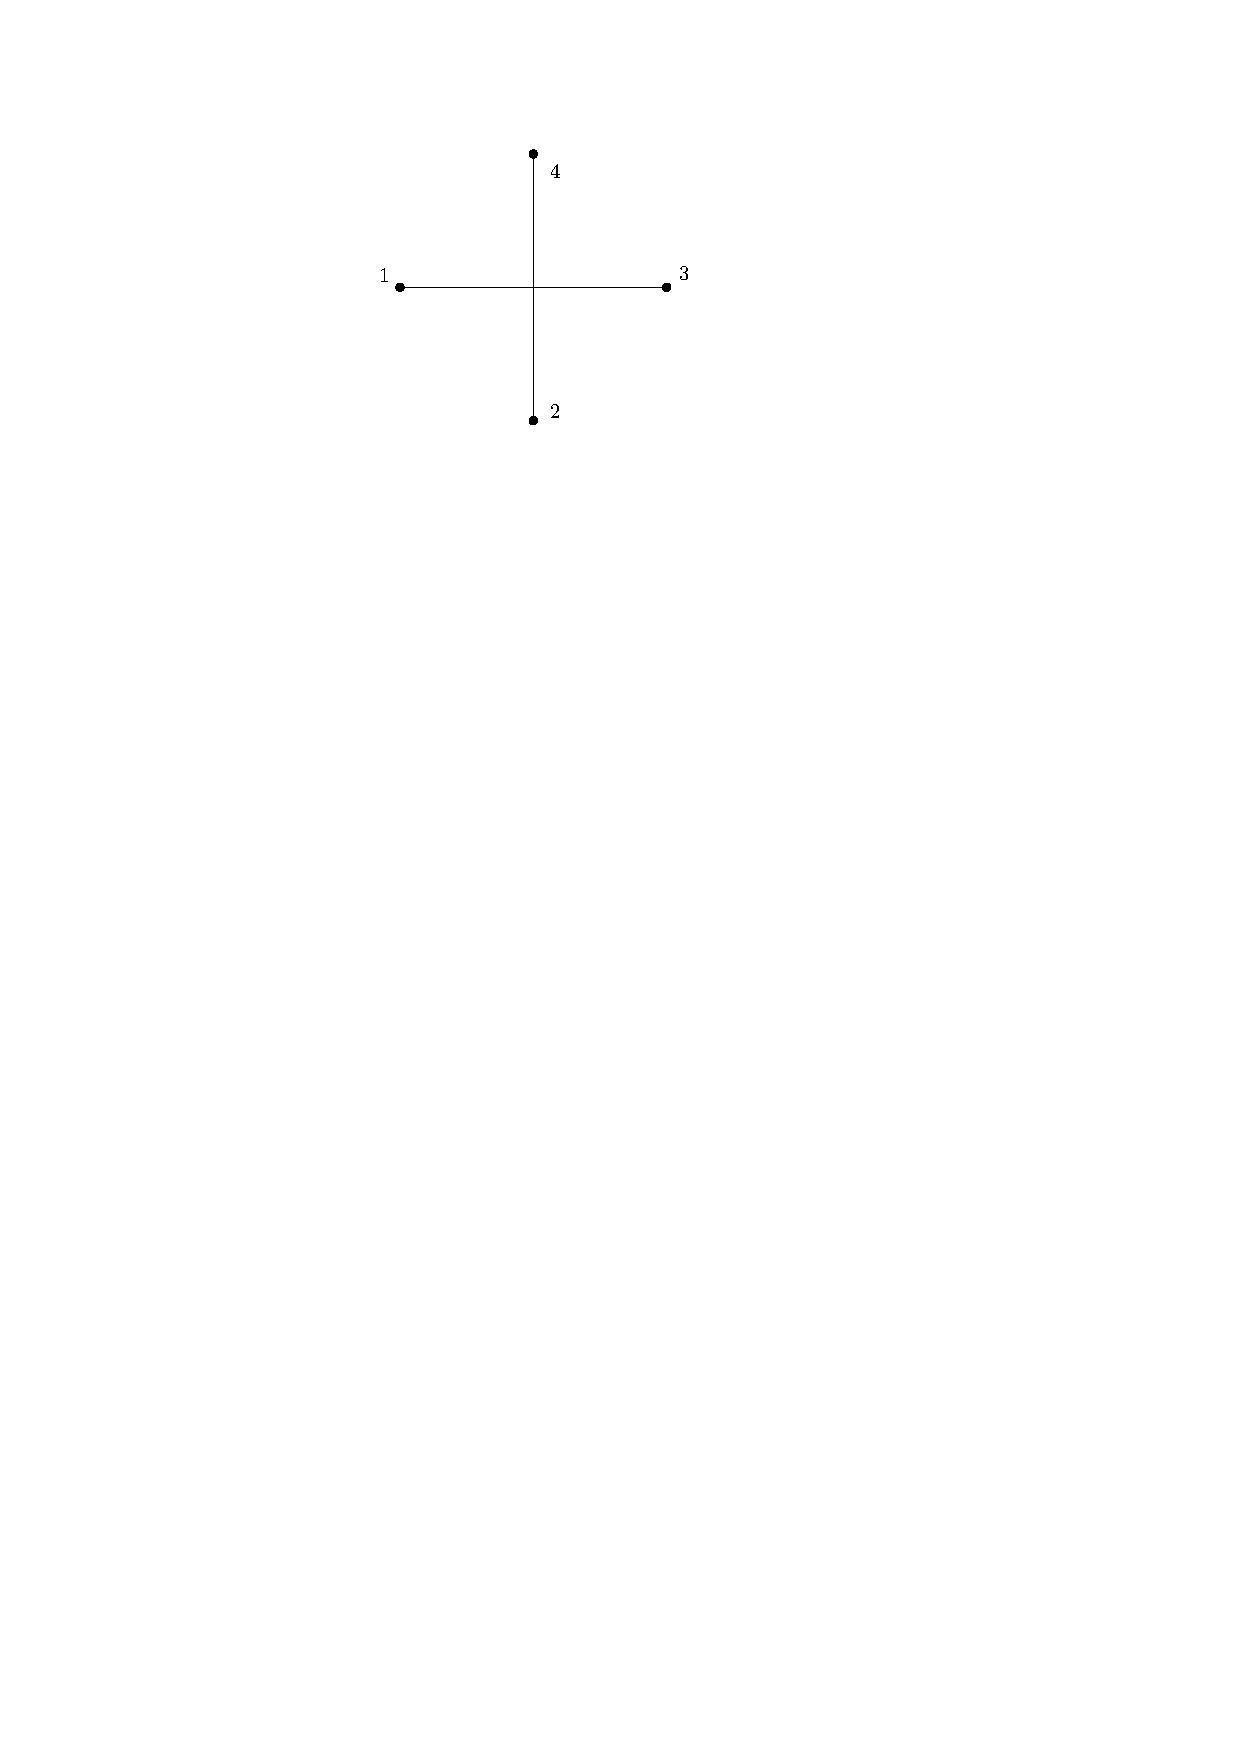
\includegraphics{graphics/crossingType2.pdf}
	  \caption{The interior of the edges intersect.}
	  \label{fig:ch1-linkages-1-2}
  \end{subfigure}
  \begin{subfigure}[b]{0.49\textwidth}
	  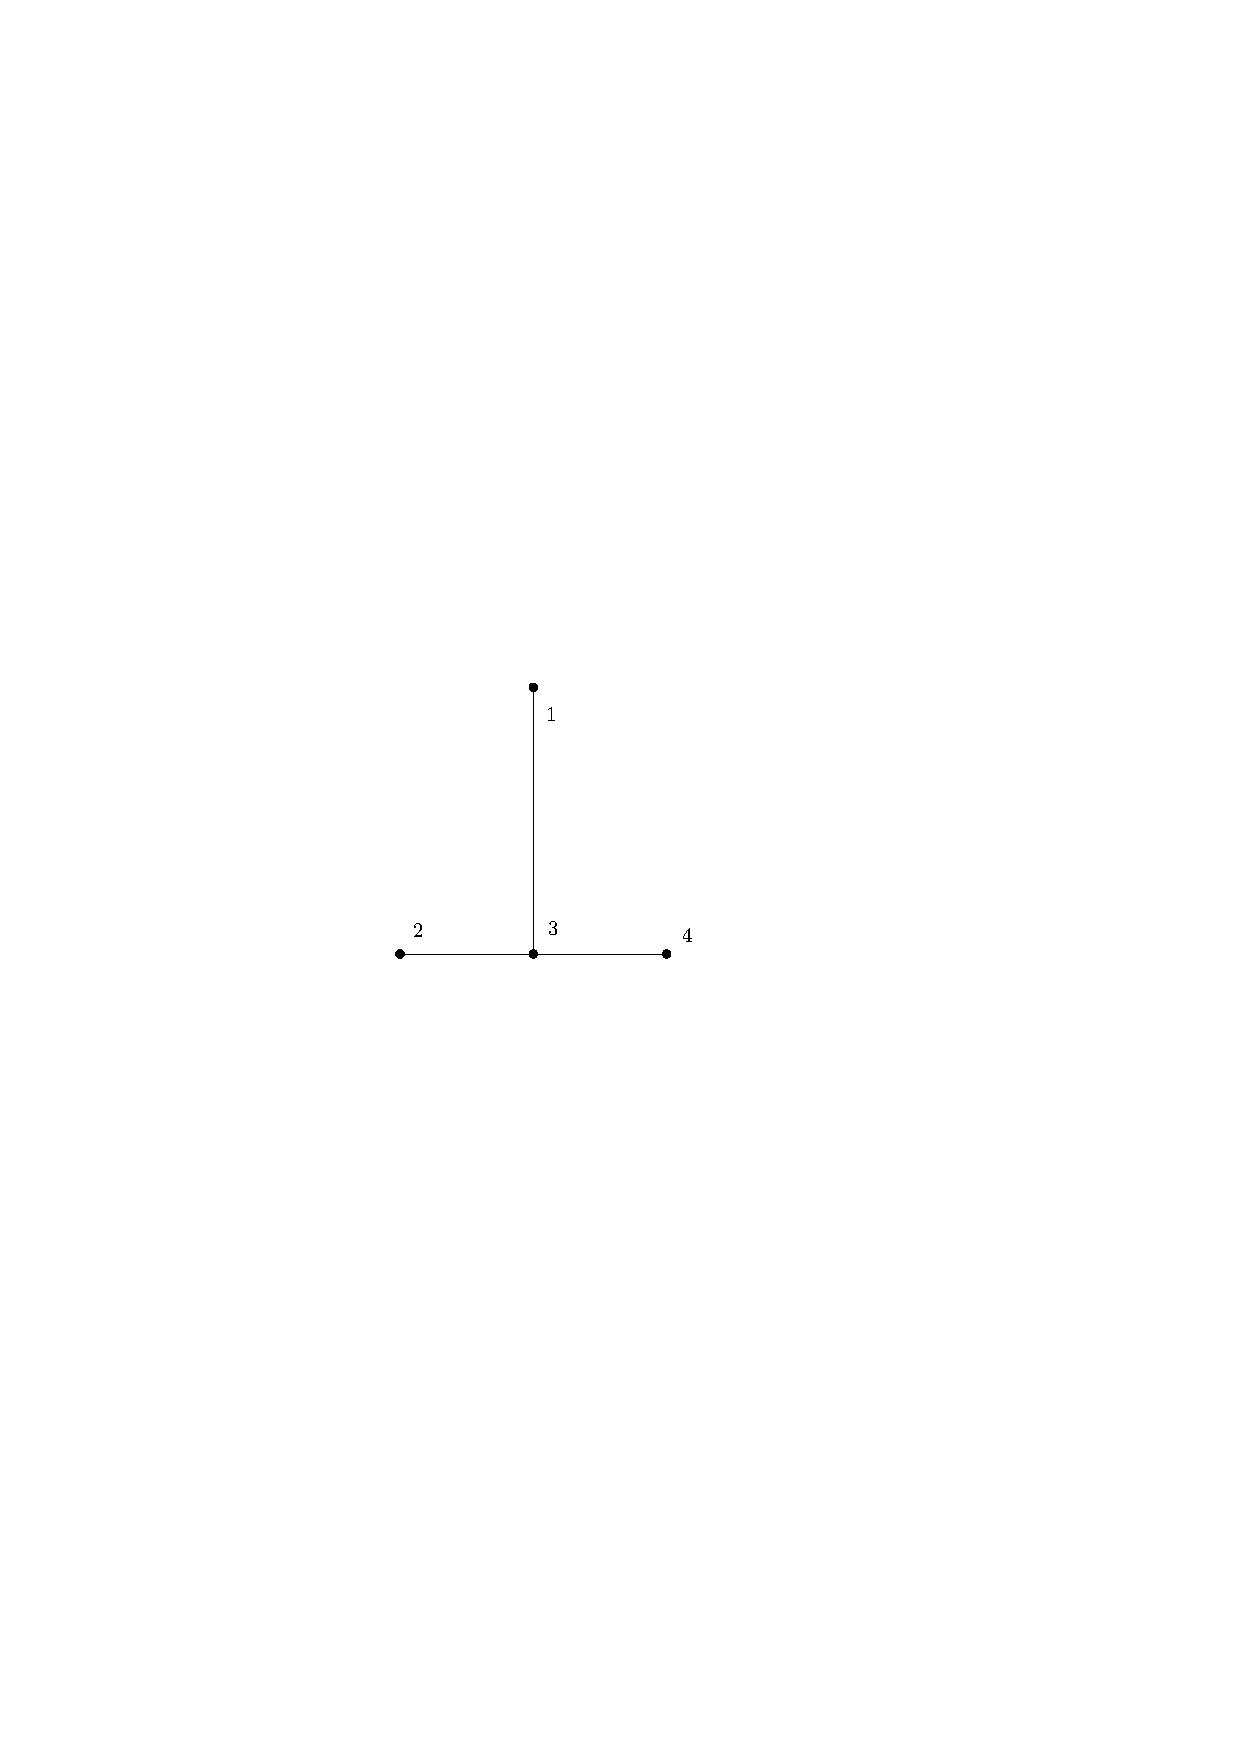
\includegraphics{graphics/crossingType3.pdf}
	  \caption{An edge passes through a vertex.}
	  \label{fig:ch1-linkages-1-3}
  \end{subfigure}
\end{center} 
\caption{These figures exhibit the 4 types of edge crossings.}\label{fig:ch1-linkages-1}
\end{figure}
A graph is called \textit{planar} if it admits a plane embedding.  A \textit{plane graph} is a 
graph together with a plane embedding.
\subsection{Trees}
A \textit{path} is a sequence of vertices in which every two consecutive vertices are connected by 
an edge.   
A \textit{simple  cycle} of a graph is a sequence, $(v_1, v_2, \dots, v_{t-1},v_t)$, of 
distinct vertices such that every two consecutive vertices are connected by 
an edge,  and the last vertex, $v_t$, connects to $v_1$.  A 
graph is \textit{connected} if for any two vertices, there exists a path between 
the two points.

A \textit{tree} is a graph that has no simple cycles and is connected.
\begin{figure}[h]
\begin{center}
  \begin{subfigure}[b]{0.49\textwidth}
    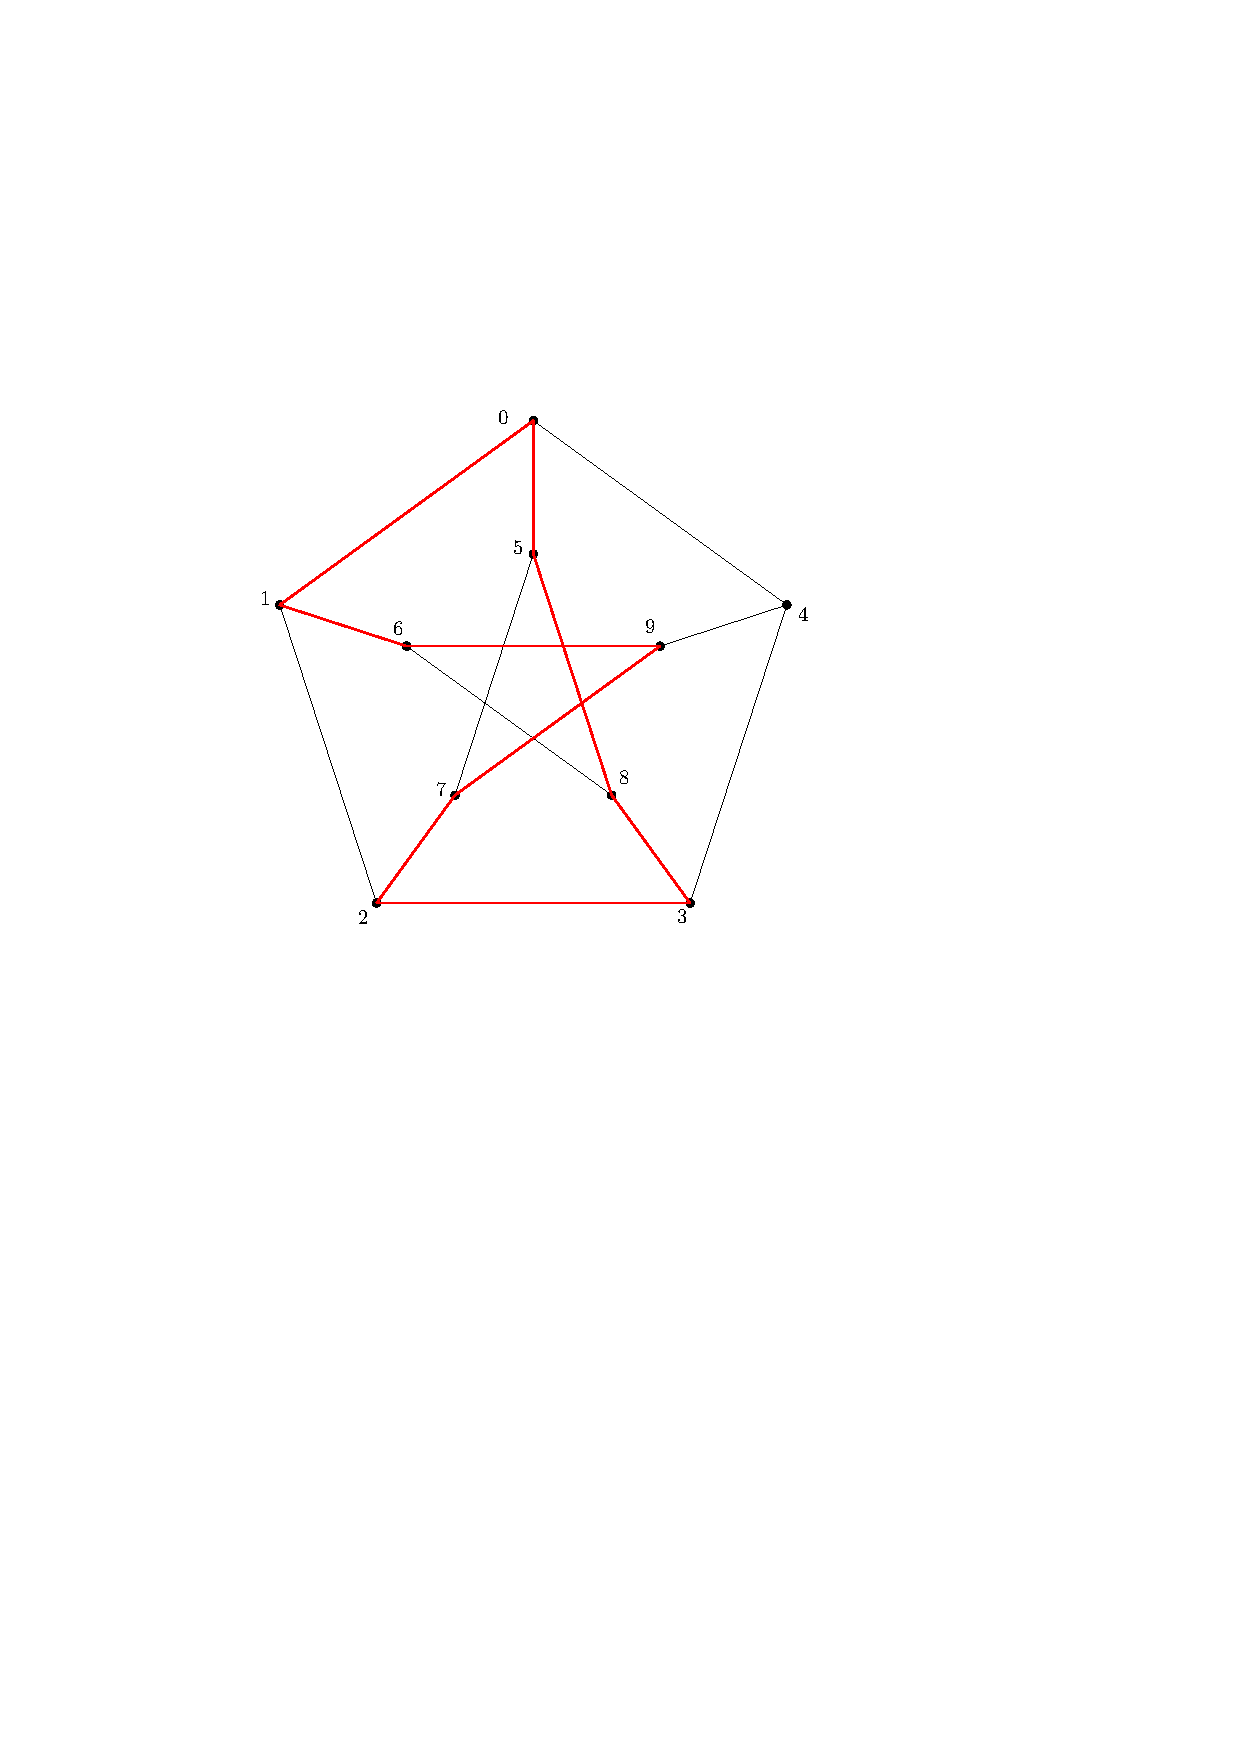
\includegraphics{graphics/PetersonGraphAgain.pdf}
    \caption{An embedding of the Peterson graph with a simple cycle of 
    (2,7,9,6,1,0,5,8,3).}\label{fig:ch1-graph-2}
  \end{subfigure}
  
\end{center}
\end{figure}
\subsection{Ordered Trees}
An \textit{ordered tree} is a tree together with a cyclic order of the neighbors for each vertex.
\begin{figure}[h]
\begin{center}
    \includegraphics{graphics/OrderedTreesExample.pdf}
    \caption{A tree with two embeddings with different cyclic orderings around 
vertices.}\label{fig:ch1-graph-6}
\end{center}
\end{figure}
Embeddings of ordered trees are equivalent if for each node the counter-clockwise ordering of 
adjacent nodes are the same.
\subsection{Graph Isomorphism} 
To determine when two graphs are equivalent, we need to define an isomorphism for graphs.  Given 
two graphs $G_1 =(V_1,E_1)$ and $G_2 = (V_2,E_2) $, a \textit{graph isomorphism} a bijective 
function $f: V_1 \mapsto 
V_2$ 
such that for any two vertices $u,v \in V_1$, we have $\{u, v\} \in E_1$, if and 
only 
if $(f(u),f(v)) \in E_2$. 
\begin{table}[!ht]
\begin{center}
$$\begin{array}{|c|c|c|}\hline
\text{Graph}&\text{Vertices}&\text{Edges}\\\hline
G_1&\left\lbrace a,b,c,d,e \right\rbrace & \left\lbrace ab,(b,c),(c,d),(d,e),(e,a) \right\rbrace 
\\\hline
G_2&\left\lbrace 1,2,3,4,5 \right\rbrace & \left\lbrace (1,2),(2,3),(3,4),(4,5),(5,1) \right\rbrace 
\\\hline
\end{array} $$
\caption{Two graphs that are isomorphic with the alphabetical isomorphism $f(a)=1$, $f(b)=2$, $f(c) 
= 3$, $f(d)=4$, $f(e)=5$.}
\end{center} 
\label{table:ch1-graph-1}
\end{table}

\begin{figure}[!h]
\begin{center}
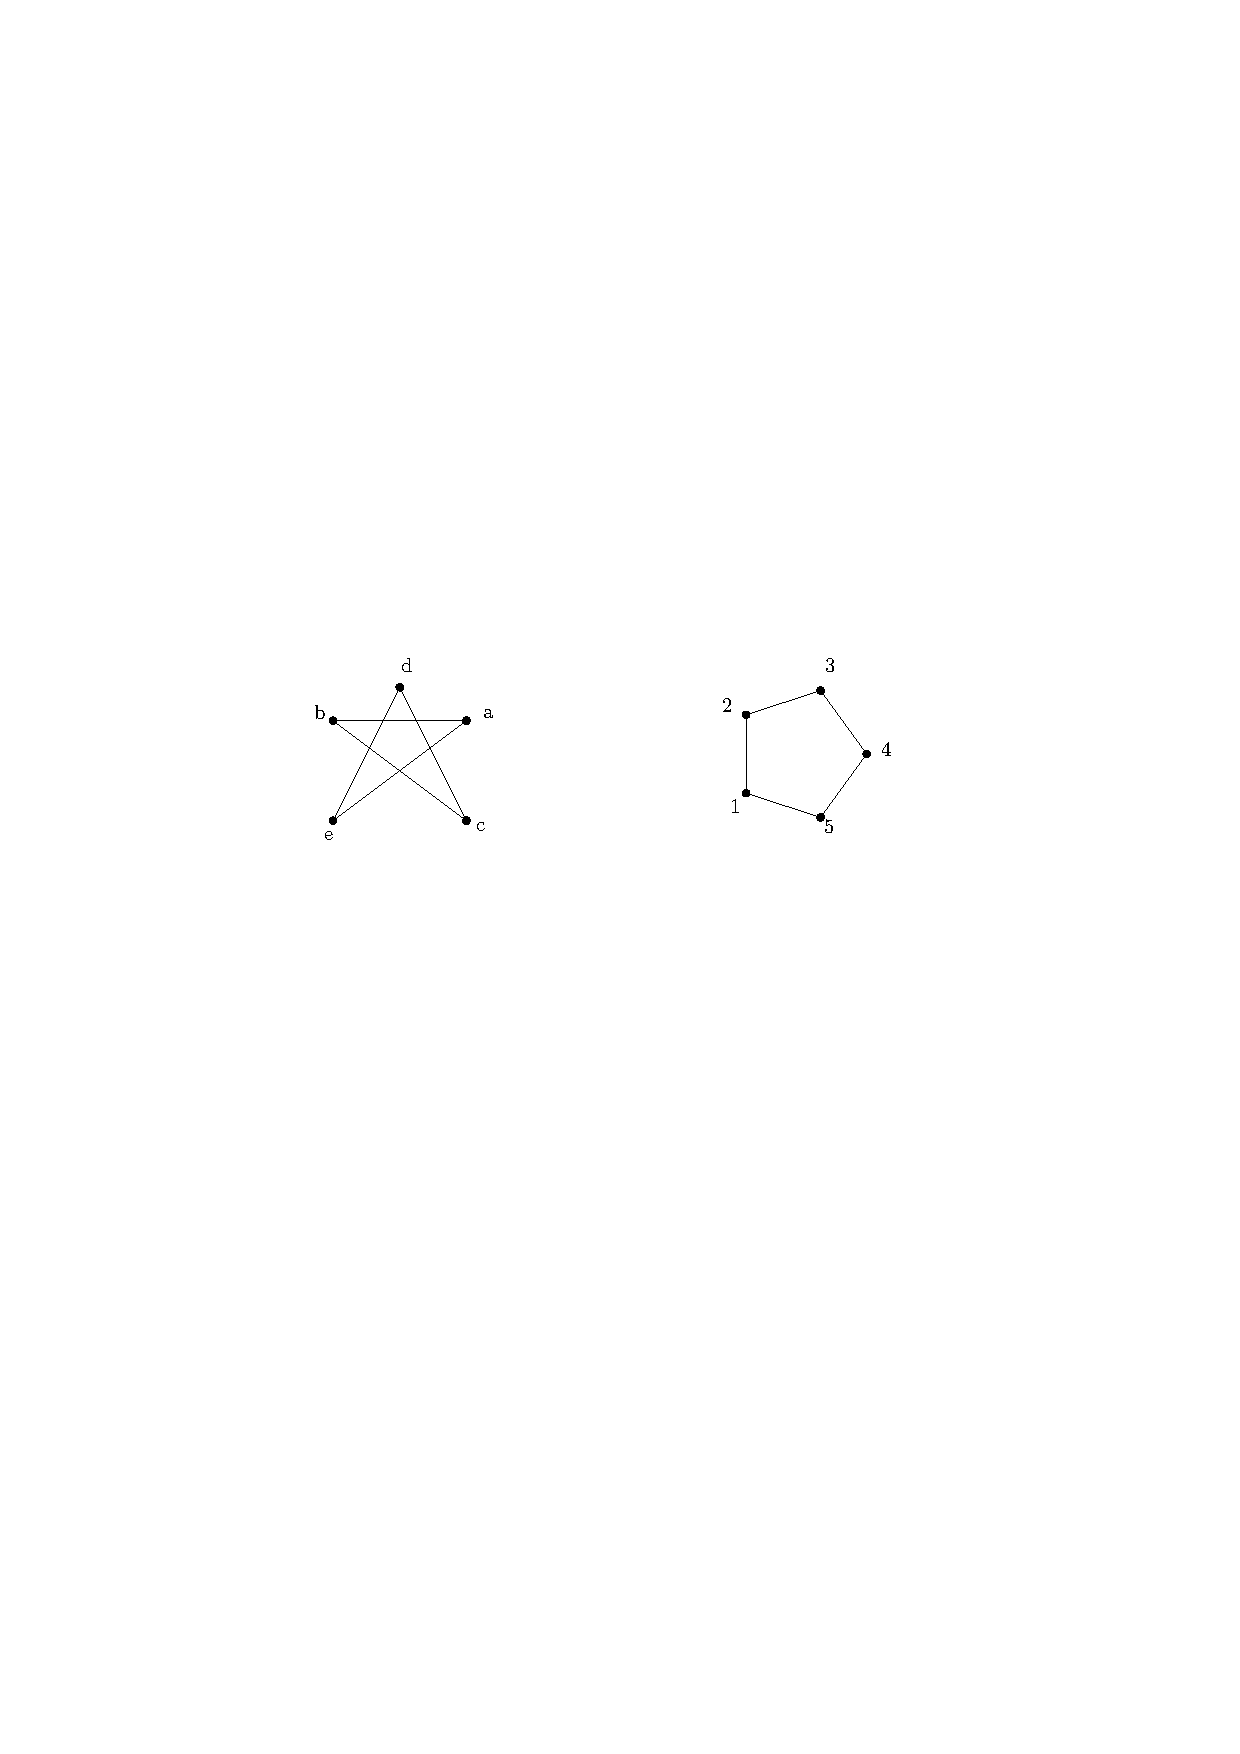
\includegraphics[scale=1]{graphics/graphIsomorphismExample.pdf}
\end{center} 
\caption{This figure depicts the graph isomorphism shown in Table 
(\ref{table:ch1-graph-1}) between 
$V_1$ and $V_2$ in the plane.}
\label{fig:configuration-3}
\end{figure}


% Next we add restrictions to our graph isomorphisms to narrow our focus:
% \begin{itemize}
% \item[\rn{1}] We focus on isomorphisms for planar graphs and or polygonal linkages, simple planar 
% graphs, and
% \item[\rn{2}] the isomorphism preserves edge lengths (polygonal area), e.g. $d(u,v) = d(f(u),f(v))$.
% \end{itemize}  
% With these restrictions of our isomorphisms, we can begin to describe a range of motion to 
% transform a linkage.  That range of motion is said to be the configuration space of that linkage.  
% To expand on this concept, for given linkage, $L=(V,E)$, and for a given vertex $v \in V$, the set 
% of points in which $v$ can be realized in the plane would be the configuration space for that 
% vertex, $C_v$.  Defining some order of the vertices in $L$, i.e. $V = \left\lbrace v_n 
% \right\rbrace_{i=1}^n$, then the \it{configuration space} for $L$ is said to be the cartesion 
% product of the configuration space of vertices:
% \subsection{Summary}
% \begin{table}[!ht]
% \begin{center}
% $$\begin{array}{|l|c|c|}
%  \hline
% &\text{Linkages}&\text{Polygonal Linkages}\\\hline
% \text{Ordered Pair}&G&G\\\hline
% \text{Edges}&E&\HH\\\hline
% \text{Vertices}&V&\PP\\\hline
% l&l&\text{N.A.}\\\hline
% \text{Embedding of }G&\Pi : V \mapsto \bbr^2&\PP ' = \left\lbrace P_i ' 
% \right\rbrace_{i=1}^n\\\hline
% \text{Realization}&\text{See (a)}&\text{See (b)}\\\hline
% \end{array}
% \caption
% $$
% \caption{(a)The realization for a linkage is for any edge $(u,v) \in E$ such that $\left\vert 
% \Pi(u)-\Pi(v)\right\vert = l(u,v)$.(b)A \emph{realization} of a polygonal linkage is an 
% interior-disjoint placement of congruent copies of the polygons in $\PP$ such that the points 
% corresponding to each hinge are identified (Fig. \ref{fig:1}, left).(c).}
% \end{center} 
% \label{table:linkages-2}
% \end{table} 
% %1) 
% %DESCRIBE THE FOLLOWING:
% %1)CONFIGURATION SPACE AS A VECTOR SPACE OF DIMENSION 2^N WHERE EDGE LENGTH IS PRESERVED.
% %2)PINNING 1 VERTEX TO ORIGIN AND A NEIGHBOR, ADD MOTIVATION TO PREVENT ROTATION AND TRANSLATIONS.
% 
% % \begin{equation}\label{eqn:linkages-1}
% % C(L) = C_{v_1} \cross C_{v_2} \cross \cdots \cross C_{v_n}
% % \end{equation} 
% % Some food for thought on configuration spaces and motions on linkages:
% % \begin{itemize}
% % \item[\rn{1}] A configuration space is said to be \it{connected} if there is a continuous mapping 
% for any two planar realizations (linkages) of a graph in the plane.  Otherwise it is said to be 
% \it{disconnected}.
% % \item[\rn{2}] If the configuration space of a vertex, $C_v$, is a singleton set, then the vertex 
% is said to be \it{pinned}. Otherwise it is said to be \it{free}.
% % \item[\rn{3}] The types of motions (mappings) that we refrain from using on linkages are 
% translations.
% % \end{itemize}
% % Note that configuration spaces for polygonal linkages are described similarly.
% % \subsubsection{Realizability of Linkages}
% % Suppose we had two configurations of a linkage, $\mathcal{A}$ and $\mathcal{B}$.  A question that 
% can be posed is can we reconfigure $\mathcal{A}$ to $\mathcal{B}$ continuously while respecting 
% simple planar graph conditions?  The answer to this question is a yes or no.  If yes, then there 
% must exist a path connected configuration space between $\mathcal{A}$ and $\mathcal{B}$.  It has 
% been shown that this problem can be posed as a planar satisfiability problem 
% \cite{Breu19983,mulzer2008minimum} (Later on in this paper we'll cover satisfiability problems).  
% This is the type of problem that we face in this paper.  We will continue to explore this in a 
% different manner, with circle packings.
% \newpage 
